% Slide 1
\section{Ứng dụng của CLIP}
\begin{frame}{5. Ứng dụng của CLIP}
\begin{itemize}
    \item \textbf{Truy vấn} giữa ảnh và văn bản (Text-to-Image, Image-to-Text Retrieval)
    \item Nâng cao: \textbf{Phân biệt khuôn mặt}, từ đó phát triển tác vụ nhận diện khuôn mặt người.
\end{itemize}
\end{frame}

\begin{frame}{5.1 Ứng dụng của CLIP trong truy vấn giữa ảnh và văn bản}
\begin{itemize}
    \item Text-to-Image, Image-to-Text Retrieval
    \item CLIP hỗ trợ truy vấn đa chiều: từ văn bản tìm ảnh, hoặc từ ảnh tìm văn bản mô tả tương ứng.
    \item Ví dụ: Gõ “người đàn ông đeo kính” → truy xuất ảnh phù hợp trong tập dữ liệu.
    \item Ứng dụng trong tìm kiếm hình ảnh, gợi ý nội dung, kiểm duyệt nội dung tự động,...
\end{itemize}
\end{frame}

\begin{frame}{5.1.1 Giới thiệu bộ dữ liệu COCO 2017}
\begin{itemize}
    \item \textbf{COCO} (Common Objects in Context) là bộ dữ liệu chuẩn cho nhiều bài toán thị giác máy tính: phát hiện đối tượng, phân đoạn ảnh, và truy xuất ảnh từ văn bản.
    
    \item \textbf{Số lượng:}
    \begin{itemize}
        \item \textbf{Train2017:} 118.000 ảnh có gán nhãn.
        \item \textbf{Val2017:} 5.000 ảnh dùng để đánh giá mô hình.
        \item \textbf{Test2017:} 41.000 ảnh (không có nhãn công khai).
    \end{itemize}

    \item \textbf{Chú thích:} Mỗi ảnh đi kèm trung bình 5 câu mô tả tự nhiên (caption) — phù hợp cho huấn luyện/truy vấn ảnh-văn bản.

    \item \textbf{Định dạng:} Ảnh '.jpg' và nhãn định dạng '.json' (COCO-style annotations).

    \item \textbf{Ứng dụng:} Được dùng rộng rãi trong huấn luyện và đánh giá mô hình như CLIP, BLIP, Flamingo, ViLT,...
\end{itemize}
\end{frame}

\begin{frame}{5.1.2 Thực hiện bài toán truy vấn với CLIP (ViT-B/32)}
\textbf{Ghi chú:} Do bài toán yêu cầu huấn luyện trên tập dữ liệu lớn và đòi hỏi tài nguyên GPU đáng kể, mô hình CLIP đã được huấn luyện sẵn bởi OpenAI là một lựa chọn phù hợp và hiệu quả.

\vspace{1em}
\textbf{Các bước thực hiện:}
\begin{itemize}
    \item \textbf{Bước 1:} Nạp mô hình CLIP ViT-B/32 được huấn luyện sẵn từ thư viện OpenAI.
    \item \textbf{Bước 2:} Tiền xử lý ảnh và văn bản đầu vào (chuẩn hóa kích thước, token hóa văn bản).
    \item \textbf{Bước 3:} Trích xuất vector đặc trưng (embedding) cho cả ảnh và văn bản thông qua mô hình CLIP.
    \item \textbf{Bước 4:} Tính độ tương đồng cosine giữa các vector đặc trưng để đo mức độ phù hợp.
    \item \textbf{Bước 5:} Truy xuất kết quả phù hợp nhất: tìm ảnh gần nhất với truy vấn văn bản, hoặc ngược lại.
\end{itemize}
\end{frame}

\begin{frame}{5.1.3 Kết quả và Nhận xét trên tập COCO}
\textbf{Kết quả đánh giá trên tập COCO validation:}
\begin{itemize}
    \item \textbf{Recall@1:} 49.92\%
    \item \textbf{Recall@5:} 74.94\%
    \item \textbf{Recall@10:} 83.24\%

\end{itemize}

\vspace{0.5em}
\textbf{Nhận xét:}
\begin{itemize}
    \item CLIP đạt kết quả tốt với Recall@10 trên 83\%, cho thấy khả năng định vị đúng ảnh nằm trong top đầu là rất cao.
    \item Recall@1 còn hạn chế ($\sim$ 50\%) – mô hình có thể nhầm khi truy vấn có ngữ nghĩa gần nhau.
    \item Phù hợp với ứng dụng cần độ bao phủ cao (top-5/top-10), cần cải tiến thêm nếu yêu cầu chính xác tuyệt đối.
\end{itemize}
\end{frame}

\begin{frame}{5.1.4 Ví dụ minh hoạ kết quả truy vấn}
\begin{columns}
    % Cột trái: hình ảnh
    \begin{column}{0.5\textwidth}
        \centering
        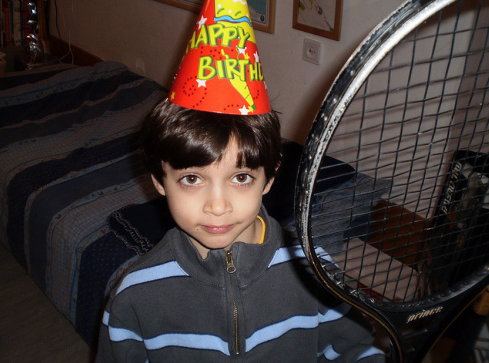
\includegraphics[width=0.95\linewidth]{img/05-imagecaption.png} % Thay bằng đường dẫn ảnh thật
        \vspace{0.5em}
        \textit{Ảnh minh hoạ truy vấn}
    \end{column}

    % Cột phải: truy vấn và caption
    \begin{column}{0.5\textwidth}
        \textbf{Truy vấn văn bản:} 
         \begin{itemize}
        \item “A boy in birthday hat holding a tennis racket” , 
        \item "A boy swinging a tennis racket at a ball on a court."
        \end{itemize}

        \vspace{1em}

        \textbf{Caption gốc:}
        \begin{itemize}
            \item “A boy in birthday hat holding a tennis racket"
            \item "A young boy in a birthday hat holds a tennis racquet”
        \end{itemize}
    \end{column}
\end{columns}
\end{frame}

\begin{frame}{5.2 Ứng dụng CLIP để phân biệt khuôn mặt người}
\begin{itemize}
    \item CLIP học mối liên hệ giữa ảnh và văn bản từ hàng trăm triệu cặp dữ liệu.
    \item Dù không thiết kế riêng cho nhận diện khuôn mặt, CLIP có khả năng biểu diễn ảnh mạnh mẽ.
\end{itemize}
\textbf{Mục tiêu}
\begin{itemize}
    \item Mã hóa ảnh khuôn mặt thành vector đặc trưng (embedding).
    \item Dự đoán và phân biệt khuôn mặt bằng cách so sánh độ tương đồng giữa các embedding.
\end{itemize}
\end{frame}

% Slide 2
\begin{frame}{5.2.1 Dữ liệu}
\textbf{Dữ liệu:} Kaggle Face Recognition Dataset
\begin{itemize}
    \item Dựa trên LFW, ảnh 250x250 JPG.
    \item Mỗi thư mục tương ứng với một người nổi tiếng (2–50 ảnh).
\end{itemize}
\textbf{Xử lý dữ liệu:}
\begin{enumerate}
    \item Tăng cường dữ liệu (augmentation).
    \item Chia thành Train/Test.
    \item Tạo Dataloader với cặp ảnh.
\end{enumerate}
\begin{figure}
    \centering
    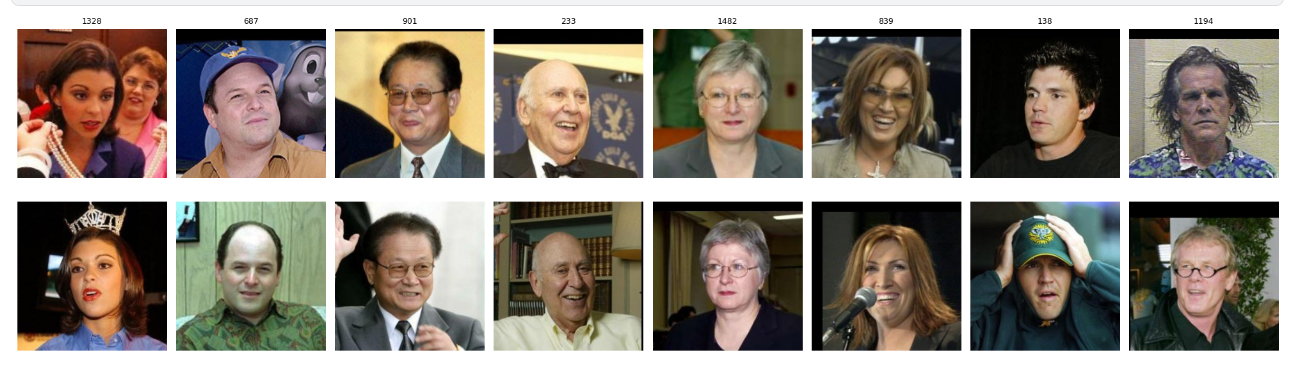
\includegraphics[width=0.75\linewidth]{img/05-Face.png}
    \caption{Ví dụ khuôn mặt trong tập dữ liệu.}
\end{figure}
\end{frame}

% Slide 3
\begin{frame}{5.2.2 Sử dụng lớp VisionTransformer từ ViT-B/32 (CLIP)}
\begin{columns}
    \begin{column}{0.62\textwidth}
        \begin{itemize}
        \item \textbf{Patch Embedding:} Ảnh chia thành các patch kích thước $32 \times 32$ và chuyển thành vector.
    \item \textbf{LayerNorm:} Chuẩn hóa đầu vào cho Transformer.
    \item \textbf{Transformer Encoder:} Gồm 12 khối ResidualAttentionBlock:
    \begin{itemize}
        \item Mỗi block có multi-head attention với đầu vào/ra 768 chiều.
        \item Chuẩn hóa (\texttt{ln\_1}, \texttt{ln\_2}).
        \item MLP: Linear(768 $\rightarrow$ 3072) $\rightarrow$ QuickGELU $\rightarrow$ Linear(3072 $\rightarrow$ 768).
    \end{itemize}
    \item \textbf{Output LayerNorm:} Chuẩn hóa để lấy embedding có đầu ra 768.
        \end{itemize}
    \end{column}
    \begin{column}{0.25\textwidth}
        \centering
        \begin{figure}
            \centering            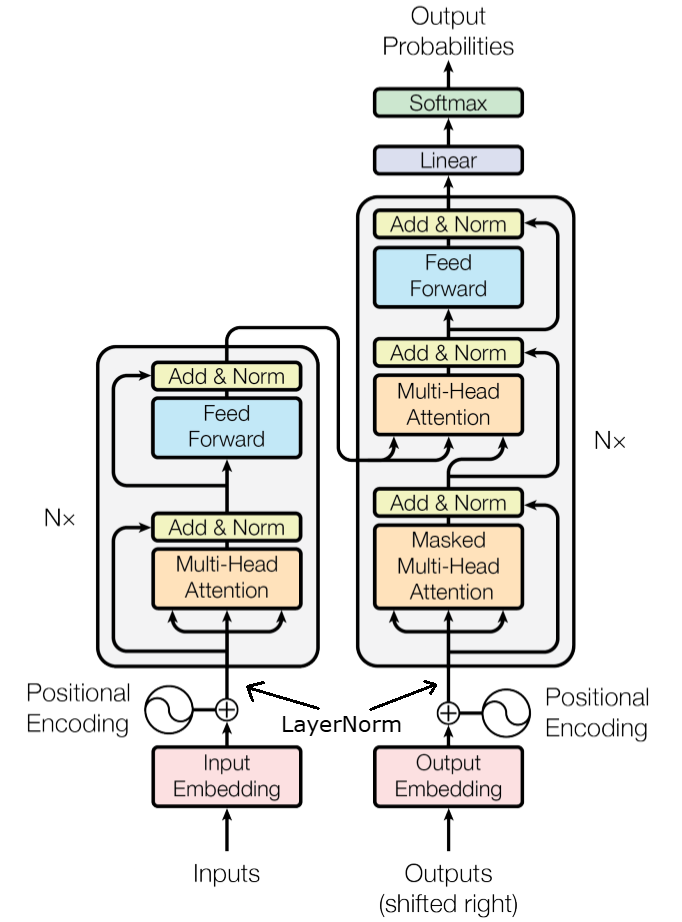
\includegraphics[width=\linewidth]{img/05-visontransformer.png} 
            \tiny Kiến trúc mạng Vision Transformer
        \end{figure}
    \end{column}
\end{columns}
\end{frame}


\begin{frame}{5.2.3 Huấn luyện và Đánh giá mô hình ViT}
\begin{columns}
    % Cột trái: mô tả
    \begin{column}{0.5\textwidth}
        \small % �� Chữ nhỏ hơn bình thường
        \begin{itemize}
            \item \textbf{Loss:} Contrastive Loss
            \item \textbf{Optimizer:} Adam (learning rate = $1 \times 10^{-3}$)
            \item \textbf{Epoch:} 3
            \item \textbf{Các cặp ảnh:} cùng người, khác người
            \item \textbf{Nhận xét:}
            \begin{itemize}
                \item Sau 3 epoch, loss giảm, mô hình chưa hội tụ. Embedding vector giữa các lớp chưa đủ tách biệt.
                \item Khả năng phân biệt ảnh khác người còn yếu, dẫn đến precision thấp trên tập test. Mô hình dễ nhầm lẫn các cặp không cùng người. F1-score ở mức trung bình cho thấy cần cải thiện thêm.
            \end{itemize}
        \end{itemize}
    \end{column}

    % Cột phải: biểu đồ + bảng
    \begin{column}{0.5\textwidth}
        \begin{figure}
            \centering
            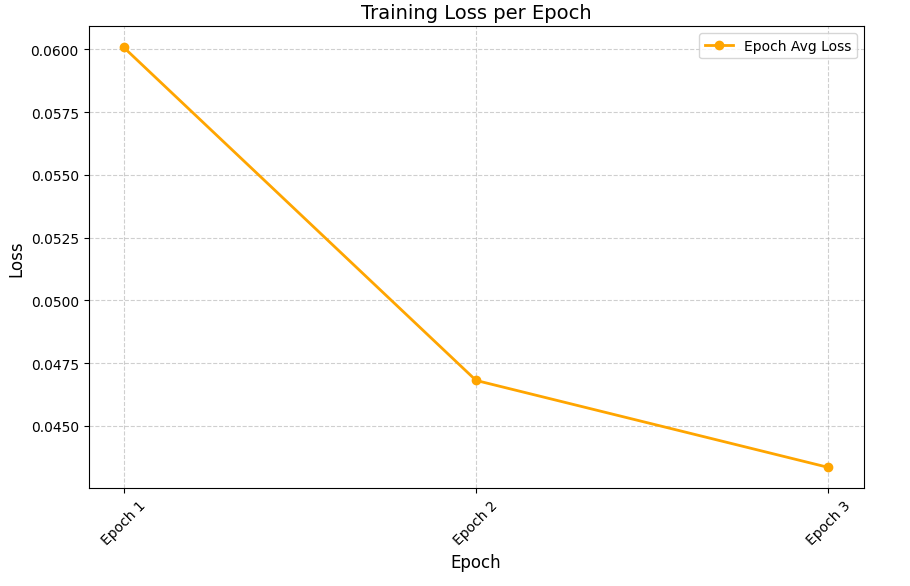
\includegraphics[width=0.8\linewidth]{img/05-loss.png}
        \end{figure}
        \begin{center}
        \scriptsize
        \begin{tabular}{|l|c|c|}
            \hline
            \textbf{Chỉ số} & \textbf{Train} & \textbf{Test} \\
            \hline
            Accuracy  & 72.92\% & 71.65\% \\
            Precision & 83.56\% & 66.76\% \\
            Recall    & 57.06\% & 86.24\% \\
            F1-score  & 67.81\% & 75.26\% \\
            \hline
        \end{tabular}
        \end{center}
    \end{column}
\end{columns}
\end{frame}

\begin{frame}{5.2.4 Kết quả ảnh test}
\vspace{-0.5em}

\begin{minipage}[t]{0.48\textwidth}
    \centering
    \begin{figure}
    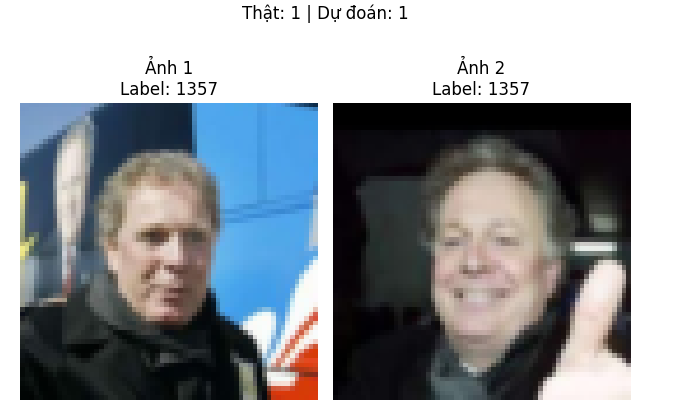
\includegraphics[width=0.95\linewidth]{img/05-1.png}
    {Khoảng cách: 0.1810\\Thật: 1, Dự đoán: 1}
    \end{figure}
\end{minipage}
\hfill
\begin{minipage}[t]{0.48\textwidth}
    \centering
    \begin{figure}
        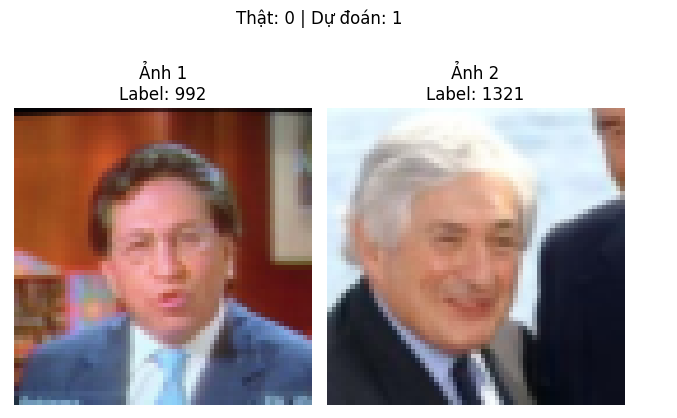
\includegraphics[width=0.95\linewidth]{img/05-2.png}
        {Khoảng cách: 0.1999\\Thật: 0, Dự đoán: 1}
    \end{figure}
        
\end{minipage}

\begin{itemize}
    \item  Tính \textbf{Khoảng cách} giữa hai vector đặc trưng ảnh.
    \item Nếu khoảng cách $<$ \textbf{0.2} thì hai ảnh được dự đoán là \textbf{cùng nhãn}.
\end{itemize}
\end{frame}


\begin{frame}{5.2.5 So sánh với mô hình CNN khác trong tác vụ phân biệt khuôn mặt người}
\footnotesize
Mặc dù không được thiết kế chuyên biệt cho tác vụ phân biệt khuôn mặt người, mô hình vẫn đạt hiệu quả cao nhờ chiến lược: \textbf{trích xuất embedding cho toàn bộ ảnh, tính khoảng cách, và gán nhãn theo ảnh gần nhất trong tập dữ liệu đã biết.}
\begin{table}[H]
\centering
\begin{tabular}{|c|c|c|c|c|}
\hline
\textbf{Mô hình} & Accuracy & Precision & Recall & F1 \\
\hline
CLIP (ViT-B/32) & \textbf{0.73} & \textbf{0.6982} & \textbf{0.7311} & \textbf{0.7022} \\
ResNet18        & 0.2151           & 0.1743           & 0.2151          & 0.1672          \\
ResNet50        & 0.2169           & 0.1493         & 0.2169          & 0.1483          \\
EfficientNet-B0 & 0.2218           & 0.1658           & 0.2218          & 0.1621          \\
MobileNetV2     & 0.2602           & 0.1916          & 0.2602         & 0.1923         \\
\hline
\end{tabular}
\end{table}
\begin{itemize}
    \item CLIP pretrained mang lại hiệu suất cao, không cần huấn luyện lại.
    \item Ưu tiên sử dụng CLIP nếu tài nguyên tính toán cho phép.
\end{itemize}
\end{frame}

